\documentclass[10pt,oneside]{article}
\usepackage{polski}
\usepackage{fancyhdr} %numerowanie i toppery
\usepackage{lastpage} %ostatnia strona
\usepackage{indentfirst} %wcięcie
\usepackage{tikz}
\usepackage{graphicx}

\title{Specyfikacja implementacyjna - BieszczadyTour}
\author{Adrian Bączek}
\date{14.11.2019}

\pagestyle{fancy}
\fancyhf{}


\begin{document}
\maketitle

\rfoot{
	\begin{flushright}
		v1.0
	\end{flushright}
}

\thispagestyle{fancy}

\newpage

\rfoot{
	\begin{center}
		Strona \thepage \hspace{1pt} z \pageref{LastPage}
	\end{center}
}

\tableofcontents

\newpage

\section{Wstęp}
\subsection{Cel dokumentu}
Celem dokumentu jest ułatwienie samodzielnego napisania kodu programu przez programistów pragnących odtworzyć działające oprogramowanie we własnym środowisku.
\subsection{Odbiorca dokumentu}
Dokument stworzony został z myślą o ludziach szukających własnej ścieżki samorozwoju, pragnących pogłębić wiedzę na temat algorytmów i istoty programowania. 

\section{Środowisko deweloperskie}
Sekcja zawiera podstawowe informacje na temat środowiska, w którym powstawało oprogramowanie, ułatwiające wierne jego lokalne odtworzenie przez odbiorcę.
\begin{center}
Parametry komputera i środowiska programistycznego:
\newline \newline
\begin{tabular}{|c|c|} \hline
	Procesor & Intel(R) Core(TM) i5-3230M CPU@2.60 GHz
	\\[10pt] Pamięć RAM & 8GB DDR3 1600 MHz
	\\[10pt] Karta graficzna & Nvidia GeForce GT 630M
	\\[10pt] System operacyjny & Windows 10 Home v10.0.18362
	\\[10pt] Język programowania & C\#
	\\[10pt] Środowisko programistyczne & Visual Studio 2019 v16.3.2 \\ \hline
\end{tabular}
\end{center}

\section{Zasady wersjonowania}
Wersjonowanie projektu w opisywanym dokumencie odbywać się będzie w~następujący sposób. Zaplanowanych zostało 10 wydań oprogramowania, kończąc implementację kodu na wersji 1.0. Według założeń projektu, aktualna wersja oprogramowania dostępna będzie w gałęzi głównej repozytorium (,,master"), zaś każdy ,,release" przygotowywany będzie na osobnej gałęzi oznaczonej odpowiednią dla siebie etykietą. Po zamknięciu prac konkretnego etapu rozwoju oprogramowania nastąpi połączenie odpowiedniej gałęzi z gałęzią główną ,,master". Zastosowanie takiej strategii prowadzenia prac umożliwi jednoczesny dostęp do stabilnej wersji oprogramowania jak i jego rozszerzania o nowe funkcjonalności.

\section{Struktura programu i diagram klas}
Rozdział opisuje dokładną strukturę modułów wchodzących w skład oprogramowania.

\subsection{Management}
Moduł odpowiedzialny za zarządzanie logiką oprogramowania. Posiada metodę główną ,,main", w której to następuje start programu.
\subsection{FileValidator}
Moduł odpowiedzialny za walidację danych podanych na wejściu przez użytkownika. Moduł posiada metody do weryfikacji poprawności formatu danych wejściowych ( CheckInputFormat() ), poprawności identyfikatora miejsca startowego ( CheckIdentifier() ) oraz spójności danych ( CheckConsistency() ).
\subsection{Graph}
Moduł zawiera model grafu, który będzie wykorzystany w wyznaczaniu szukanej trasy podróży. Atrybutem instancji tej klasy jest prywatna lista węzłów wchodzących w skład analizowanego grafu. Potrzebny obiekt tworzony będzie na podstawie listy połączeń otrzymanej z instancji klasy ,,FileValidator".
\subsection{Node}
Moduł zawiera model pojedynczego elementu grafu. Według założeń każdy węzeł posiada prywatny identyfikator oznaczający ID miejsca do odwiedzenia, prywatną listę połączeń oraz nazwę miejsca na trasie. 
\subsection{NodeConnection}
Moduł zawiera format w jakim przechowywane będą połączenia grafu w~programie. Powiązania węzłów zaprojektowane są tak by reprezentowały połączenie dwóch jednostek w grafie skierowanym tzn. zawierają referencję do węzła docelowego oraz informację o koszcie i czas drogi z punktu A do punktu B. Zarówno czas jak i koszt będą reprezentowane przez liczby zmiennoprzecinkowe typu float. 
\subsection{PathOptimiser}
Moduł odpowiadający za główną część programu. Posiada jedną metodę wyznaczającą optymalną ścieżkę podróży.

\begin{figure}
	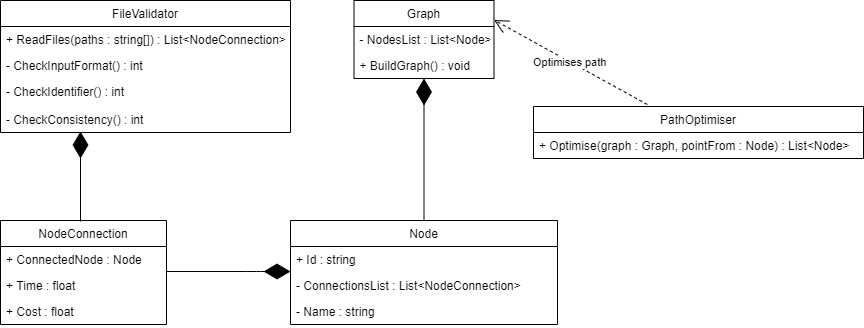
\includegraphics[scale=0.5]{diagram_klas.png}
	\caption{Diagram klas stosowanych w programie ,,BieszczadyTour".}
\end{figure}

\section{Rozwiązanie zadania}
Zadaniem realizowanym przez program jest nic innego jak zmodyfikowany problem komiwojażera. Na wstępie warto ująć, iż jest to problem który charakteryzuje się dużą złożonością obliczeniową - O(n!). Z tego względu stosowane są algorytmy proponujące rozwiązania w dużym stopniu tak dobre jak rozwiązanie optymalne. Jednym z nich jest powtarzalny algorytm najbliższego sąsiada. Wyznaczone przez niego ścieżki są gorsze od optymalnej zaledwie o 25\%. Biorąc pod uwagę klasę problemu (problem komiwojażera jest NP-trudny) można stwierdzić iż algorytm ten w zupełności wystarczy do wyznaczania trasy podróży.

\subsection{Schemat działania algorytmu}
 Poniższą sekwencję kroków wykonujemy dla każdego wierzchołka rozważanego grafu.
\newline
\begin{enumerate}
	\item Wybrany przez nas wierzchołek grafu obierany jest jako aktualny, po czym zaznaczamy go jako wierzchołek odwiedzony.
	\item Przeglądamy listę połączonych wierzchołków z aktualnym i wybieramy połączenie o najmniejszej wadze.
	\item Dopisujemy do rozwiązania krawędź łączącą wierzchołek aktualny i ostatnio wybrany.
	\item Oznaczamy dołączony wierzchołek jako odwiedzony i przyjmujemy jako aktualny.
	\item W przypadku istnienia niedołączonych wierzchołków przechodzimy do punktu 2.
	\item Znajdujemy najkrótszą ścieżkę od aktualnego wierzchołka do wierzchołka obranego w punkcie 1.
	\item Aktualizujemy wybraną najlepszą trasę.
\end{enumerate}

\subsection{Informacje o zastosowanym algorytmie}
\begin{center}
	Zestawienie podstawowych informacji o użytym w programie algorytmie
	\newline \newline
	\begin{tabular}{|c|c|} \hline
		Złożoność obliczeniowa & O($n^{3}$)
		\\[10pt] Złożoność pamięciowa & O($n^{2}$) \\ \hline
	\end{tabular}
\end{center}

\end{document}
